\documentclass{article}
\usepackage[utf8]{inputenc}
\usepackage[T1]{fontenc}
\usepackage{babel}
\usepackage{listings}
\usepackage{xcolor}
\usepackage{tikz}
\usetikzlibrary{arrows,
                positioning,
                quotes,
                shapes}
\lstset{language=C++,
                frame=single,
                basicstyle=\ttfamily,
                keywordstyle=\color{blue}\ttfamily,
                stringstyle=\color{red}\ttfamily,
                commentstyle=\color{green}\ttfamily,
                morecomment=[l][\color{magenta}]{\#}
}
\newcommand{\nodes}[1]{%
    \foreach \num [count=\n starting from 0] in {#1}{% no need for an external counter
      \node[minimum size=3mm, draw, circle,fill=black!10] (n\n) at (\n,0) {\textbf{\num}};
    }
}
\tikzstyle{arrow} = [thick,->,>=stealth]
\tikzstyle{dashedarrow} = [dashed,->,->=stealth]
\begin{document}
\title{ \textbf{Union Find}}
\author{Niccolò Piazzesi\\n.piazzesi@studenti.unipi.it}
\maketitle
\begin{abstract}
The Union Find data structure, also called Disjoint Set Union (DSU) is a very interesting data structure, not 
only  for the algorithmic techniques and  analysis involved, but also for its applications, especially to graph problems. In this
report I will present a high level view of UnionFind, describing the fundamental structure and the various implementations. In the last section, I will also present
a collection of problems for which the use of a DSU provides an efficient solution.
\end{abstract}
\section{Description}
Suppose we have a collection S of \emph{n} distinct elements, let's say the integers from 1 to \emph{n}. 

Initially these elements
are organized in n disjointed sets \{1\},\{2\},...,\{n\}. For simplicity we will assume that the name of set \{i\}
is i. In the union find problem we want to mantain a collection of disjointed sets while supporting the following operations:
\begin{itemize}
    \item \textbf{union}(A, B): join the sets A and B in a single set. The name of the new set is A and the old sets A and B are destroyed.
    \item \textbf{find}($x$): given an element $x$, return the name of the set that contains it.
\end{itemize}
Let's now generalize the problem. We have assumed before that the n elements are already given. This is not true in general, so we need a way to 
add new elements (and consequentially new sets). This is solved by introducing a third operation:
\begin{itemize}
    \item \textbf{makeSet}($x$): Create a new set {$x$} containing the single element $x$. The name of the new set is $x$.
\end{itemize}
We will say that the UnionFind problem consists of mantaining a collection of disjointed sets during 
an arbitrary sequence of \emph{makeSet, union} and \emph{find} operations, starting from the empty set \cite{demetrescu}. Figure \ref{fig:circle} shows a
simple example where the elements considered are numbers. For the rest of the report we will consider a unionFind problem with
$n$ makeSet operations and $m$ find operations. Since we have a total of n disjointed sets, we don't have to specify the number
of union operations, because they cannot be more than $n-1$.

\begin{figure}
    \centering

    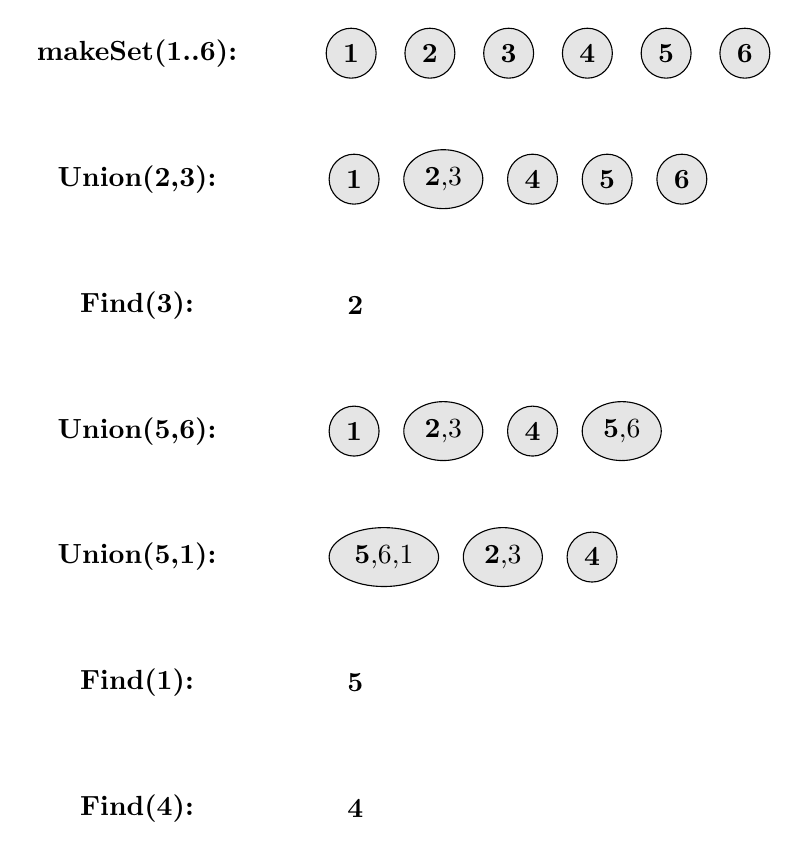
\begin{tikzpicture}
    
    \nodes{1,2,3,4,5,6}
    
    \node[minimum size = 3mm](start)[left=1cm of n0]{\textbf{makeSet(1..6):}};
    \node[minimum size=3mm] (u1)[below=of start] {\textbf{Union(2,3):}};
    \node[circle,fill=black!10, draw, minimum size=3mm] (u1n1)[right=1.3cm of u1] {\textbf{1}};
    \node[ellipse,fill=black!10,draw,fill=black!10, minimum size=3mm] (u1n2)[right=0.3cm of u1n1] {\textbf{2},3};
    \node[circle,fill=black!10, draw, minimum size=3mm] (u1n3)[right=0.3cm of u1n2] {\textbf{4}};
    \node[circle,fill=black!10, draw, minimum size=3mm] (u1n4)[right=0.3cm of u1n3] {\textbf{5}};
    \node[circle,fill=black!10, draw, minimum size=3mm] (u1n5)[right=0.3cm of u1n4] {\textbf{6}};
    
    \node[minimum size=3mm] (f1) [below= of u1]{\textbf{Find(3):}};
    \node[minimum size=3mm] (f1n1)[right=1.7cm of f1]{\textbf{2}};
    
    \node[minimum size=3mm] (u2)[below=of f1] {\textbf{Union(5,6):}};
    \node[circle,fill=black!10, draw, minimum size=3mm] (u2n1)[right=1.3cm of u2] {\textbf{1}};
    \node[ellipse,fill=black!10,draw, minimum size=3mm] (u2n2)[right=0.3cm of u2n1] {\textbf{2},3};
    \node[circle,fill=black!10, draw, minimum size=3mm] (u2n3)[right=0.3cm of u2n2] {\textbf{4}};
    \node[ellipse,fill=black!10,draw, minimum size=3mm] (u2n4)[right=0.3cm of u2n3] {\textbf{5},6};
    
    \node[minimum size=3mm] (u3)[below=of u2] {\textbf{Union(5,1):}};
    \node[ellipse,fill=black!10,draw, minimum size=3mm] (u3n1)[right=1.3cm of u3] {\textbf{5},6,1};
    \node[ellipse,fill=black!10,draw, minimum size=3mm] (u3n2)[right=0.3cm of u3n1] {\textbf{2},3};    
    \node[circle,fill=black!10, draw, minimum size=3mm] (u3n3)[right=0.3cm of u3n2] {\textbf{4}};
    
    \node[minimum size=3mm] (f2) [below= of u3]{\textbf{Find(1):}};
    \node[minimum size=3mm] (f2n1)[right=1.7cm of f2]{\textbf{5}};

    \node[minimum size=3mm] (f3) [below= of f2]{\textbf{Find(4):}};
    \node[minimum size=3mm] (f3n1)[right=1.7cm of f3]{\textbf{4}};
    
    \draw [arrow] (u2) (u2n1);
    \end{tikzpicture}
    
    \caption{A running example with 6 initial elements. The name of each set is written in bold}
    \label{fig:circle}
\end{figure}

\section{Naive Implementations}
The general idea for implementing UnionFind is to consider the collection as a forest of trees, with each tree represeting a single set. 
In the following code we will only consider integers as elements and use an array representation of the forest.
Given an array \emph{parents} the element \emph{parents[i]} contains the direct parent of element \emph{i} in the tree hierarchy. For the root
r of a tree we will have parents[r] $=$ r. Before analyzing a more efficient implementation, we will see two simpler versions.
\newpage
\subsection{QuickFind}
\begin{figure}[h!]
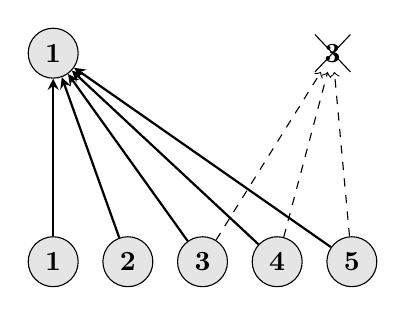
\begin{tikzpicture}
    \node[circle,fill=black!10, draw=, minimum size=3mm] (qf1) at (0,0) {\textbf{1}};
    \node[circle,cross out, draw, minimum size=3mm] (qf2)[right= 3cm of qf1] {\textbf{3}};
    \node[circle,fill=black!10, draw, minimum size=3mm] (qf3)[below= 2cm of qf1] {\textbf{1}};
    \node[circle,fill=black!10, draw, minimum size=3mm] (qf4)[right= 0.3cm of qf3] {\textbf{2}};
    \node[circle,fill=black!10, draw, minimum size=3mm] (qf5)[right= 0.3cm of qf4] {\textbf{3}};
    \node[circle,fill=black!10, draw, minimum size=3mm] (qf6)[right= 0.3cm of qf5] {\textbf{4}};
    \node[circle,fill=black!10, draw, minimum size=3mm] (qf7)[right= 0.3cm of qf6] {\textbf{5}};

    \draw [arrow] (qf3) -- (qf1);
    \draw [arrow] (qf4) --(qf1);
    \draw [arrow] (qf5) --(qf1);
    \draw [arrow] (qf6) --(qf1);
    \draw [arrow] (qf7) --(qf1);
    \draw [dashedarrow] (qf5) -- (qf2);
    \draw [dashedarrow] (qf6) -- (qf2);
    \draw [dashedarrow] (qf7) -- (qf2);
\end{tikzpicture}
\caption{Union(1, 3) using QuickFind}
\label{fig:quickFind}
\end{figure}
\begin{center}
    \lstinputlisting[language=C++,caption=Quickfind,label=lab:qf]{code/quickFind.cpp} 
\end{center}

\subsection{QuickUnion}
\begin{center}
    \lstinputlisting[language=C++,caption=test,label=test]{code/quickUnion.cpp} 
\end{center}
\section{Balancing Heuristics}
\section{Time complexity and proof}
\section{Applications}
\bibliographystyle{plain}
\bibliography{bib}
\end{document}